\section{IR of Industrial Compilers}
\frame{
\frametitle{IR of Industrial Compilers :: LLVM Bitcode \\
How to generate IR for while statements?
}
\begin{columns}
\begin{column}{0.60\textwidth}
\begin{center}
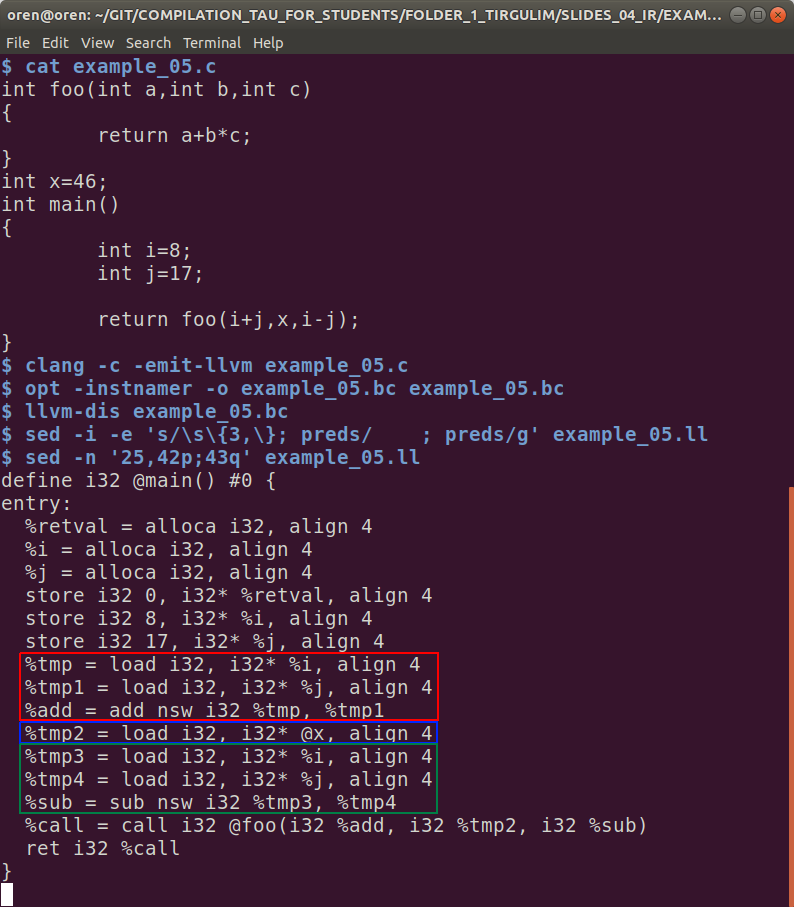
\includegraphics[width=0.95\textwidth]{example_05.png}
\end{center}
\end{column}
\begin{column}{0.6\textwidth}
\begin{itemize}
\item
three labels are created:
\begin{itemize}
\item while.cond ({\color{red} red})
\item while.body ({\color{blue} blue})
\item while.end ({\color{green} green})
\end{itemize}
\item
how to make sure \\
these labels are unique?
\item
one \textit{conditional} branch is issued
from \textit{while.cond} to either \textit{while.body}
or \textit{while.end}
\item
the other (unconditional) branch \\
is from \textit{while.body} to \textit{while.cond}
\item
What would be the only     \\
difference when generating \\
IR for if statements?
\end{itemize}
\end{column}
\end{columns}
}